\begin{center}

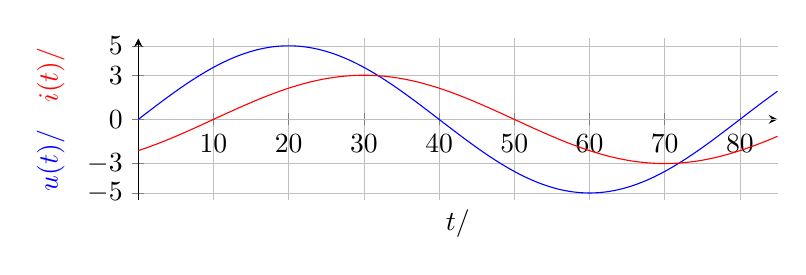
\begin{tikzpicture}
    \begin{axis}[
        domain=0:85,
        xmin=0, xmax=85,
        ymin=-5.5, ymax=5.5,
        samples=500,
        axis y line=center,
        axis x line=middle,
        xtick distance=10,
        ytick distance=1,
        extra y ticks=0,
        width=.8\textwidth,
        height=.3\textwidth,
        x label style={at={(axis description cs:0.5,0)},anchor=north},
        y label style={at={(axis description cs:-.1,.5)},rotate=90,anchor=south},
        ytick={-5,-3,0,3,5},
%         yticklabels={$-2 u_0$, $2 u_0$},
        xlabel={$t/\ms$},
         ylabel={{\color{blue}$u(t)/\volt$}\quad{\color{red}$i(t)/\ampere$}},
        grid=both,
        grid style={line width=.1pt, draw=gray!10},
        major grid style={line width=.2pt,draw=gray!50}    ]
        \addplot+[color=blue,mark=none] {5*sin(deg(x/80*6.283))};
        \addplot+[color=red,mark=none] {3*sin(deg((x-10)/80*6.283))};
    \end{axis}
\end{tikzpicture}
\end{center}